\documentclass[journal, a4paper]{IEEEtran}

\usepackage{graphicx}
\usepackage{caption}
\usepackage{subcaption}
% some very useful LaTeX packages include:

%\usepackage{cite}
\usepackage{graphicx}
\usepackage{amsmath,eqparbox,booktabs,xparse}
\usepackage{smartdiagram}
\usetikzlibrary{quotes}
%\usepackage{psfrag}   
%\usepackage{subfigure}
\usepackage{neuralnetwork}
\usepackage{url}        % Written by Donald Arseneau
\usepackage{xcolor}
\usepackage{listings}

\lstset{basicstyle=\ttfamily, keywordstyle=\bfseries}
\usetikzlibrary{arrows.meta, positioning}
\tikzset{%
    block/.style = {draw=gray, rectangle, thick,
        minimum height=6em, text width=4em, align=center}
}

\makeatletter
\NewDocumentCommand{\eqmathbox}{o O{c} m}{%
  \IfValueTF{#1}
    {\def\eqmathbox@##1##2{\eqmakebox[#1][#2]{$##1##2$}}}
    {\def\eqmathbox@##1##2{\eqmakebox{$##1##2$}}}
  \mathpalette\eqmathbox@{#3}
}
% Your document starts here!
\begin{document}

% Define document title and author
	\title{Project 1 of Deep Learning\\ \textit{\Large{Classification, weight sharing, auxiliary losses}}}
	\author{Francis \textbf{Damachi} - Costanza \textbf{Volpini}}
	\markboth{Project 1 - Deep Learning EE559 - EPFL}{}
	\maketitle
	
\begin{abstract}
The aim of this project was to show the impact of weight sharing and the use of an auxiliary loss. The task was to compare two digits represented as a two-channel image. We have started experimenting with a linear model and, then, we have implemented more complex non-linear and convolutional models. Our experiments show that, indeed, the use of weight sharing, i.e. convolutional layers, and the use of two losses leads to the best solution in his classification problem, achieving an error rate slightly higher than 15\%.
\end{abstract}

\section{Introduction}
\label{sec:intro}
\textit{Convolutional neural network} (CNN) represents the most effective architectures to analyse images because, differently than linear models, they allow to keep the shape of the input samples, which, in turn, by the use of weight sharing, allows to exploit the pixel locality to learn better.
Simple linear models were used at the beginning of the project, in particular \textit{Linear Regression} and \textit{Logistic Regression} (see Section \ref{sec:linearmodel}), we have obtained an accuracy of around $70\%$ (these models do not consider the pixel locality). Then, we have used more complex \textit{Linear Neural Networks} respectively with one-loss and two-losses (as explained and showed in Section \ref{sec:nnmodel}). With these we have got a better accuracy ($80\%$), but we were just using linear layers. Our goal, was to try to take advantage by the locality of the pixel (we want to analyze the images as whole to exploit the locality of the pixels). Therefore, the last model architecture we have tried is a \textit{Convolutional neural network} with which we could improve the accuracy ($82-84\%$) (see Section \ref{sec:cnnmodel}).

In all models, we have used \textit{Adam's method} instead of \textit{Stochastic Gradient Descent (SGD)} as optimizer since it uses a adaptive learning rates, while the SGD has a single, fixed, learning rate for all the weights/parameters of the model \cite{reference0}.
As criterion, we have used \textit{Mean Square Error} and we also show that this loss can be effectively used in a classification problem only if the output of the model is bounded, e.g. by the use of a sigmoid function.

Section \ref{sec:data} explains the structure of the dataset, Section \ref{sec:codestruc} describes briefly the content of each file. Section \ref{sec:auxilaryloss} explain which auxiliary loss we have used. In Section \ref{sec:comparison} and \ref{sec:conclusion} we have showed the performance accuracy obtained by each model using a cross validation, explaining why we got these results.


\section{Data}
\label{sec:data}
Both the train and the test sets consist of $1000$ samples. Each input sample is a tensor of shape $2\times14\times14$ tensor and represents 2 images in grayscale. While each target sample is represented by 2 tensors: (1) a single value tensor representing the boolean prediction (greater than), and (2) a two values tensor representing the classes of the two digits. The MNIST data set is made of handwritten digits (from $0$ to $9$); to load the dataset we have used the provided function \texttt{generate\_pair\_sets(N)}.

\section{Code structure}
\label{sec:codestruc}
This section describes the content of each file.
\begin{itemize}
    \item \texttt{code/data.py}: class to generate the dataset. Contains different methods (e.g. flat the input, get a dataset in 2D or in 3D, enable the hot-encoding).
    \item \texttt{code/model.py}: general class to define a model to train and test it (with corresponding plot and history).
    \item \texttt{code/models\_implemented.py}: contains all the model classes (e.g. NNModel1Loss, CNNModel2Loss).
    \item \texttt{main.py}: contains examples of each model, in order to call and train it.
\end{itemize}
Files \texttt{code/cross\_validation\_report.py} and \texttt{BoxPlot\_generator.ipynb} are made for report purposes.

The models implementation consists of an abstract class that acts as super class and implements all the common functionalities which are shared by the different models, e.g. a \texttt{fit()} function. Then, we have implemented a class for each model which defines two architectures: (1) a feature extractor, used to process the input and extract high level features, (2) one or more classifier(s) (depending on the number of losses that have been used) that are used to obtain either boolean (greater than) or digit predictions.

\section{Models}
In this section we explain the various architectures we have implemented. For each architecture we provide an image detailing its structure. In each image, we differentiate in blue the part that we called "feature extractor" and in red the parts that we treat as classifiers.

\subsection{Linear Models}
\label{sec:linearmodel}
We have implemented \textit{Linear Regression},  showed in Fig. \ref{fig:linearregression}, and \textit{Logistic Regression}, showed in Fig. \ref{fig:logisticregression}. In the logistic regression we have used a sigmoid as an activation function as final layer. A linear layer accepts as input a vector of values for each sample, therefore, the input samples have been flattened since our raw input sample are overlaid images. Therefore, the linear layer assigns a weight to each pixel. In short, in our case, the input of the linear models is a tensor of shape $(N, 2 \times 14 \times 14)=(N, 392)$, where N is the number of samples. The risk of using linear layer models is that they bad generalize images and may and up "memorizing" the train images therefore leading to overfitting, i.e. good train accuracy but a very low test accuracy.

We have observed that Linear Regression has a strange behavior during training due to the fact that it does not have a sigmoid and the loss MSE works very bad in a classification task when the output is unbounded because the MSE can easily end up penalizing a lot also correct predictions.

\begin{figure}[!h]
    \centering
    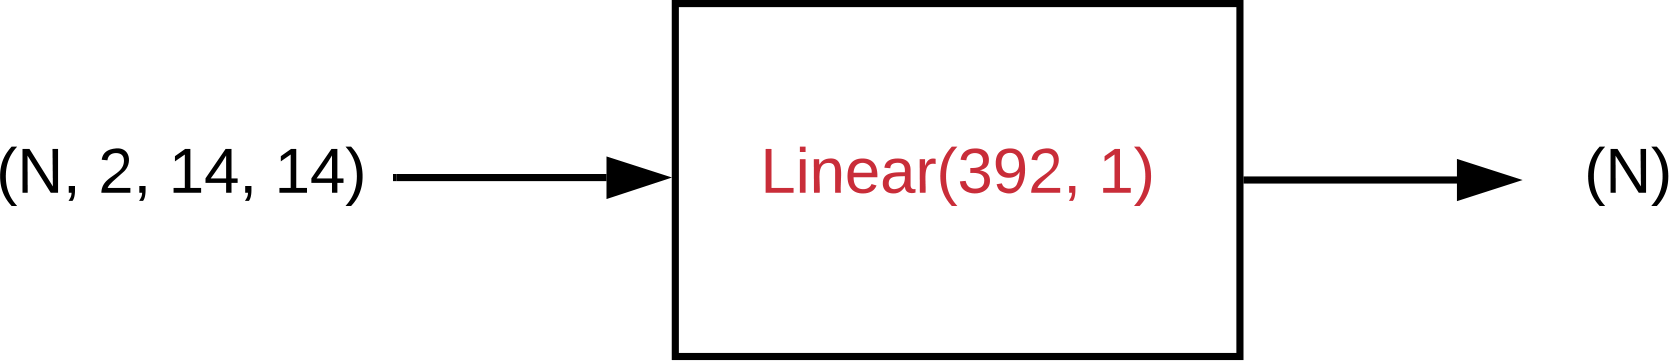
\includegraphics[width=0.35\textwidth]{linearregression.png}
    \caption{Linear Regression model}
    \label{fig:linearregression}
\end{figure}

\begin{figure}[!h]
    \centering
    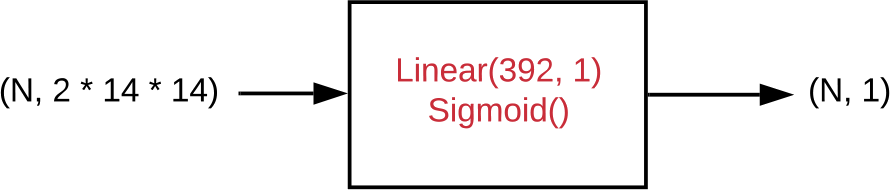
\includegraphics[width=0.35\textwidth]{logistic.png}
    \caption{Logistic Regression model}
    \label{fig:logisticregression}
\end{figure}

\subsection{Neural Network Models}
\label{sec:nnmodel}
We have implemented two models for neural network, the first one with 1 loss and the second one with 2 losses, as showed in Fig. \ref{fig:nn1} and Fig. \ref{fig:nn2}. Both models use the same feature extractors but they differs for the classifier(s). The first one has a boolean classifier that compares the two digits visible in the two images. The second model, it has also a digit classifier that returns the corresponding digit for both the handwritten images. Note that for the digit classification we have used the hot encoding to give a target to each node of he output layer.
As with the previously explained linear models, the inputs are flattened to obtain a vector of features for each sample.
Since the feature extractor processes both images together (it does not consider the two images independently), we decided to use a digit classifier with $20$ nodes as output ($10$ nodes for each digit; i.e. from $0$ to $9$ as value of digit). We have noticed that NN with 2 losses seems to perform slightly worse during the test than the model with 1 loss (see Table \ref{table:accuracy}). This is in contrast with what we were expecting. However, we believe that the use of two losses can improve the performance of the model only if the latter is more powerful enough, otherwise it can negatively affect the accuracy (as in our case). We could have improved the computation considering both the images independently, i.e. processing them independently but with the same network.

\begin{figure}[!h]
    \centering
    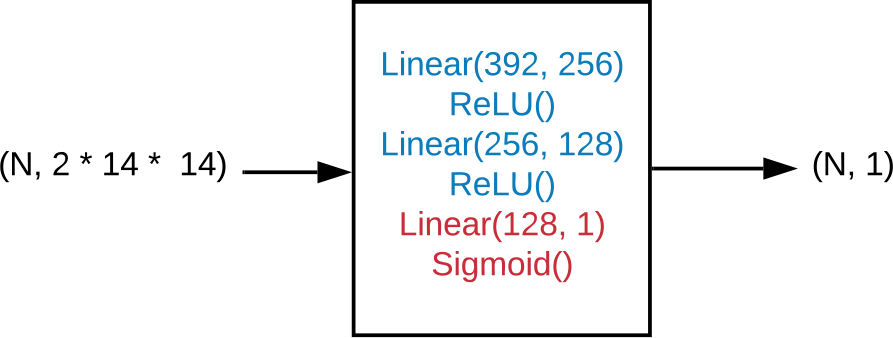
\includegraphics[width=0.35\textwidth]{nn1.png}
    \caption{Neural Network model (1 loss)}
    \label{fig:nn1}
\end{figure}

\begin{figure}[!h]
    \centering
    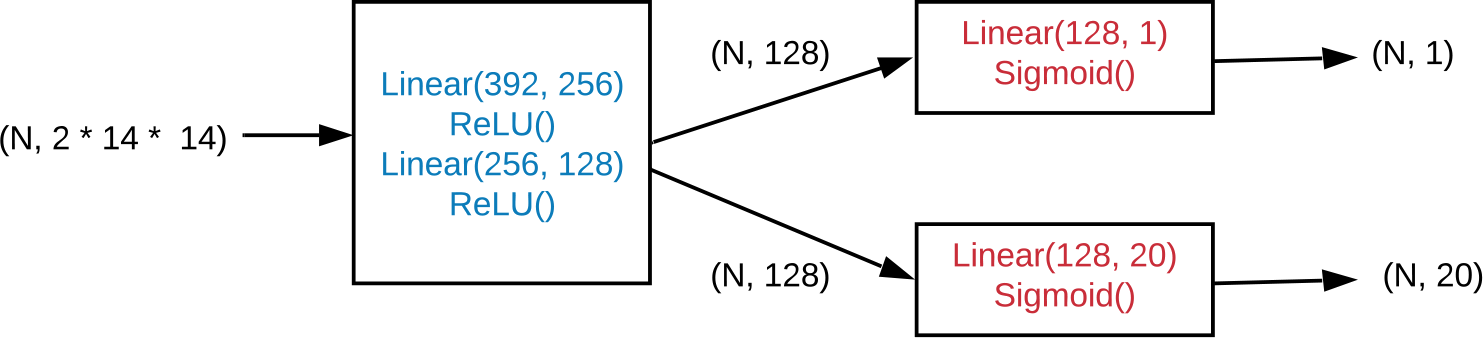
\includegraphics[width=0.5\textwidth]{nn2.png}
    \caption{Neural Network model (2 losses)}
    \label{fig:nn2}
\end{figure}


\subsection{Convolutional Neural Network Models}
\label{sec:cnnmodel}
Finally, we have decided to implement convolutional neural networks. CNNs are powerful since they use pixel locality and weight sharing. In particular, instead of flattening the input, as done for the previously explained models, we can keep the original shape of the images. Moreover, we have decided to employ \textit{conv3d} since they allow to automatically process both the images independently without the need of any preprocessing, i.e. the filters not only slide along the x and y axes but also along the z axis (in which we have our two images). As done with the model of NN, in Sec. \ref{sec:nnmodel}, we have decided to compare two models one with one loss and the other one with two losses (see Fig. \ref{fig:cnn1} and Fig. \ref{fig:cnn2}). 
We have used the dropout to generalize better and then obtain a more robust model. CNN with 2 losses got the best accuracy with $84\%$  (see Table \ref{table:accuracy}).
\begin{figure}[!h]
    \centering
    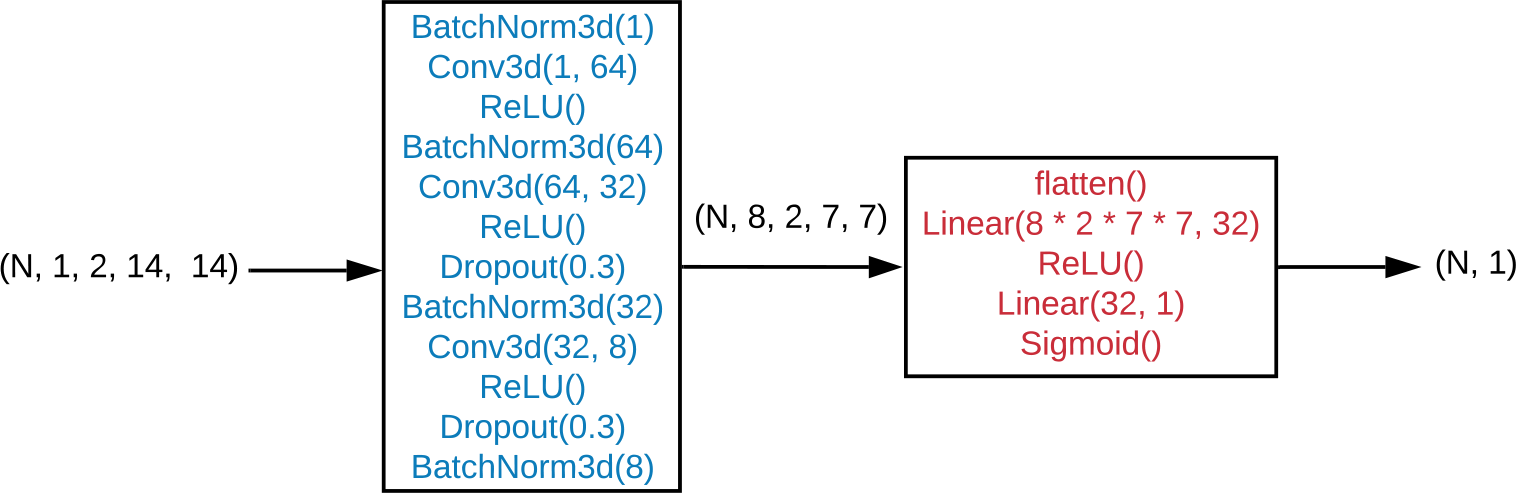
\includegraphics[width=0.5\textwidth]{cnn1.png}
    \caption{Convolutional Neural Network model (1 loss)}
    \label{fig:cnn1}
\end{figure}
\begin{figure}[!h]
    \centering
    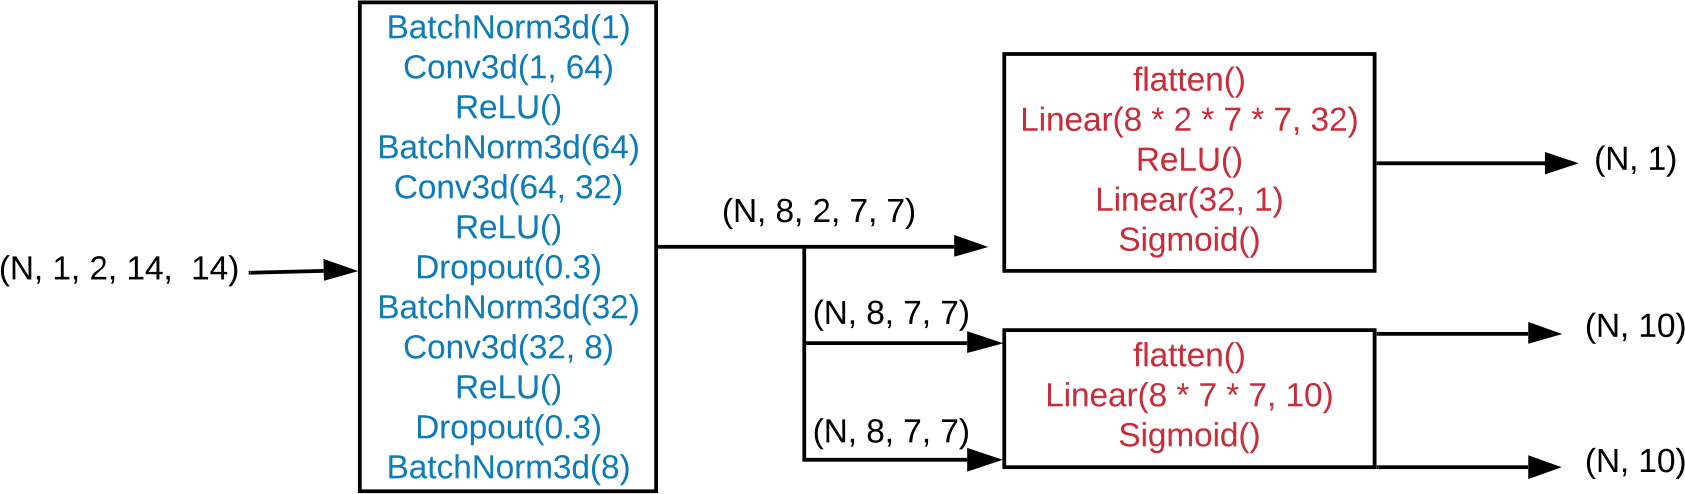
\includegraphics[width=0.5\textwidth]{cnn2.png}
    \caption{Convolutional Neural Network model (2 losses)}
    \label{fig:cnn2}
\end{figure}

\section{Comparison of models}
\label{sec:comparison}
We have decided to use cross validation to obtain a more robust comparison of the models (note that we have implement our cross validation with the library \textit{sklearn}).
Table \ref{table:params} summarizes all the number of parameters for each model. As expected neural employ weight sharing. Convolutional neural networks use weight sharing (a weight for all the pixels of the same filter) and, therefore, they require a lower number of parameters to get a good accuracy.

Box-plots have been used to show, for each model, the accuracies obtained during the cross validation (see Fig. \ref{fig:train_acc_box}). We can notice that the accuracy can vary a lot in simple models since they are very sensible to the initialization of the weights.
Moreover, we observe that the use of an auxiliary loss improved by $2\%$ the accuracy of the CNN model.

\begin{figure}[!h]
    \centering
    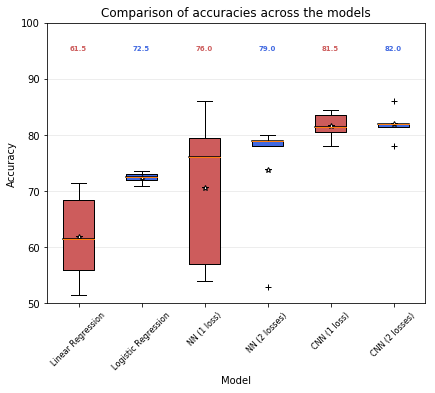
\includegraphics[width=0.5\textwidth]{boxplot.png}
    \caption{Plotbox that show the accuracy using cross validation. Star symbols represent the average values.}
    \label{fig:train_acc_box}
\end{figure}

\begin{table}
\centering
\caption{Table with number of parameters for each model.}
\label{table:params}
\begin{tabular}{|l|l|l|} 
\cline{3-3}
\multicolumn{1}{l}{} &                     & \textbf{Parameters}  \\ 
\cline{3-3}
\hline
                     & Linear Regression  & 393     \\ 
\cline{2-3}
               & Logistic Regression & 393     \\ 
\cline{2-3}
 \textbf{Models}   & NN (1 loss)~        & 133633  \\ 
\cline{2-3}
                     & NN (2 losses)~      &  136213  \\ 
\cline{2-3}
                     & CNN (1 loss)~       & 47803   \\ 
\cline{2-3}
                     & CNN (2 losses)     & 51733   \\
\hline
\end{tabular}
\end{table}

Table \ref{table:accuracy} shows the comparison between the accuracy obtained during the cross validation and the one in test. We can notice that test accuracies are higher because, while we have used the whole train set to obtain the final models and compute the test accuracy, during the cross validation the train set was divided in 5 splits and only 4 of them have been used for the training.
\begin{table}
\centering
\caption{Table accuracy (Cross validation: mean $\pm$ std).}
\label{table:accuracy}
\begin{tabular}{|l|l|l|l|} 
\cline{3-4}
\multicolumn{1}{l}{} &                     & \multicolumn{2}{c|}{\textbf{Accuracy}}  \\ 
\cline{3-4}
\multicolumn{1}{l}{} &                     & Cross validation & Test                 \\ 
\hline
                     & Linear Regression   & $61.8\pm7.467$    & $69.2$                 \\ 
\cline{2-4}
     & Logistic Regression & $72.4 \pm0.860$    & $73.8$                 \\ 
\cline{2-4}
\textbf{Models}    & NN (1 loss)~        & $70.5 \pm12.696$   & $80.5$                 \\ 
\cline{2-4}
                     & NN (2 losses)~      & $73.8 \pm10.419$   & $78.4$                 \\ 
\cline{2-4}
                     & CNN (1 loss)~       & $81.6 \pm2.289$    & $81.7$                 \\ 
\cline{2-4}
                     & CNN (2 losses)      & $81.9 \pm2.538$    & $83.7$                 \\
\hline
\end{tabular}
\end{table}

\section{Conclusion}
\label{sec:conclusion}
Convolutional Neural Network represents the best model with images recognition. Moreover, the CNN with 2 losses seems to perform slightly better since it learned to extract high-lever feature representing the two digits. We have seen that weight sharing (CNN) improves the accuracy and the robustness of the model, the use of an auxiliary loss in this context improves the obtained results.

% As future improvement we would like to implement the cross validation using the \textit{pytorch} library.
% %%%%%%%%%%%%%%%%%%%%%




% Now we need a bibliography:
\begin{thebibliography}{999}

	%Each item starts with a \bibitem{reference} command and the details thereafter.
	\bibitem{reference0}
    	optim.Adam vs optim.SGD. Let’s dive in.
    	\url{https://medium.com/@Biboswan98/optim-adam-vs-optim-sgd-lets-dive-in-8dbf1890fbdc}
	
% 	\bibitem{reference1}
% 	    Neural networks and deep learning, Michael Nielsen.
	    
%     \bibitem{reference2}
%     Notes of course Deep Learning (EE-559), Prof. François Fleuret.

\end{thebibliography}

% Your document ends here!
\end{document}

% \begin{table}
% \centering
% \caption{Table with number of parameters for each model.}
% \label{table:params}
% \begin{tabular}{|l|l|l|l|l|} 
% \cline{3-5}
% \multicolumn{1}{l}{} &                     & \multicolumn{3}{c|}{\textbf{Parameters}}          \\ 
% \cline{3-5}
% \multicolumn{1}{l}{} &                     & Feature extractor & Classifier & Total   \\ 
% \hline
%                      & Linear Regression   & -                 & 393        & 393     \\ 
% \cline{2-5}
%               & Logistic Regression & -                 & 393        & 393     \\ 
% \cline{2-5}
%  \textbf{Models}   & NN (1 loss)~        & 133504            & 129        & 133633  \\ 
% \cline{2-5}
%                      & NN (2 losses)~      & 133504            & 129        & 136213  \\ 
% \cline{2-5}
%                      & CNN (1 loss)~       & 22650             & 25153      & 47803   \\ 
% \cline{2-5}
%                      & CNN (2 losses)      & 22650             & 25153      & 49773   \\
% \hline
% \end{tabular}
% \end{table}